% !TeX root = ba.tex
\appendix
\section*{Appendices}
\addcontentsline{toc}{section}{Appendices}
\renewcommand{\thesubsection}{\Alph{subsection}}

\subsection{Detailed Description of Neural Network Architectures}
\label{lab:networks}

The following tables describe the structure of the neural networks we used in detail. Each row represents a layer (for brevity's sake some types of layers are merged into a single row).
The tables for the CapsNets are separated into two parts: The encoder network (top) and the decoder network (bottom).
Some expressions may need further explanation:

\begin{itemize}
	\item BN: spatial batch normalization
	\item Conv $K$ $F \times F$, \{valid,same\}: Convolutional layer with $F$ filters of shape $F \times F$ and either valid padding (i.e. no padding) or same padding (appropriate padding, such that output height and width is equal to that of the input)
	\item FC $n$: Fully connected with $n$ units
	\item Densely Connected: A densely connected block \citep{denselyconnected} contains multiple layers in such a way, that the input for each layer the concatenated output of all previous layer in this block is.
\end{itemize}
\todo{Explain tables (BN, Dense...)}

\begin{table}
	\centering
	
	\begin{tabular}{lc}
		\toprule 
		Layer	&  Output Shape \\ 
		\midrule 
		Conv $64$ $9\times9$, valid, ReLU, BN & $24\times24\times64$ \\ 
		\midrule 
		Primary Conv Caps, $32$ $9\times9$, dim=$8$, stride=2	&  $8\times8\times32\times8$ \\ 
		\midrule 
		Class Caps, dim=16	& $10\times16$ \\ 
		\midrule 
		& \\
		\midrule
		FC 512, ReLU	& 512 \\
		\midrule
		FC 1024, ReLU	& 1024 \\
		\midrule
		FC 784, sigmoid	& 784 \\
		\bottomrule
	\end{tabular} 
	\caption{CapsNet on MNIST}
	\label{tab:capsnet:mnist}

	\vspace{0.75cm}
	
	\begin{tabular}{lc}
		\toprule 
		Layer	&  Output Shape \\ 
		\midrule 
		Conv $32$ $5\times5$, same,	ReLU & $28\times28\times32$ \\ 
		\midrule 
		Max-Pooling $2\times2$, Dropout 0.15, BN	&  $14\times14\times32$ \\ 
		\midrule 
		Conv $64$ $3\times3$, same, ReLU	& $14\times14\times64$ \\ 
		\midrule 
		Max-Pooling $2\times2$, Dropout 0.15, BN	& $7\times7\times64$ \\
		\midrule
		Conv $128$ $3\times3$, same, ReLU	& $7\times7\times128$ \\
		\midrule
		Dropout 0.15, BN	& $7\times7\times128$ \\
		\midrule
		FC 1024, ReLU, Dropout 0.5 & 1024 \\
		\midrule
		FC 10 & 10\\
		\bottomrule
	\end{tabular} 
	\caption{ConvNet on MNIST}
	\label{tab:convnet:mnist}
\end{table}


\begin{table}
	\centering
	
	\begin{tabular}{lc}
		\toprule
		Layer	& Output Shape \\ 
		\midrule 
		Conv $32$ $3\times3$, valid, ReLU, BN	&  $26\times26\times32$ \\ 
		\midrule 
		Conv $32$ $3\times3$, valid, Leaky ReLU, BN	&  $24\times24\times32$\\ 
		\midrule 
		Primary Conv Caps, $16$ $9\times9$, dim=$8$	stride=$2$ &  $8\times8\times16\times8$\\ 
		\midrule 
		Class Caps, dim=$16$	&  $10\times16$\\ 
		\midrule 
		& \\
		\midrule
		FC 512, ReLU	& 512 \\
		\midrule
		FC 1024, ReLU	& 1024 \\
		\midrule
		FC 784, sigmoid	& 784 \\
		\bottomrule
	\end{tabular}
	\caption{CapsNet on Fashion-MNIST}
	\label{tab:capsnet:fashion}
	
	\vspace{0.75cm}
	
	\begin{tabular}{lc}
		\toprule 
		Layer	&  Output Shape \\ 
		\midrule
		Conv $32$ $5\times5$, same,	ReLU & $28\times28\times32$ \\ 
		\midrule
		Max-Pooling $2\times2$, Dropout 0.15, BN	&  $14\times14\times32$ \\ 
		\midrule 
		Conv $64$ $3\times3$, same, ReLU	& $14\times14\times64$ \\ 
		\midrule 
		Max-Pooling $2\times2$, Dropout 0.15, BN	& $7\times7\times64$ \\
		\midrule
		Conv $128$ $3\times3$, same, ReLU	& $7\times7\times128$ \\
		\midrule
		Dropout 0.15, BN	& $7\times7\times128$ \\
		\midrule
		FC 1024, ReLU, Dropout 0.5 & 1024 \\
		\midrule
		FC 10 & 10\\
		\bottomrule
	\end{tabular} 
	\caption{ConvNet on Fashion-MNIST}
	\label{tab:convnet:fashion}
\end{table}


\begin{table}
	\centering
	
	\begin{tabular}{lc}
		\toprule 
		Layer	& Output Shape \\ 
		\midrule 
		Conv $64$ $5\times5$, valid, ReLU, BN	&  $28\times28\times64$ \\ 
		\midrule 
		Conv $256$ $5\times5$, valid, Leaky ReLU, BN	&  $24\times24\times256$\\ 
		\midrule 
		Primary Conv Caps, $64$ $9\times9$, dim=$8$	stride=$2$ &  $8\times8\times64\times8$\\ 
		\midrule 
		Class Caps, dim=$16$	&  $10\times16$\\ 
		\midrule
		& \\
		\midrule
		FC 2048, ReLU	& 2048 \\
		\midrule
		FC 4096, ReLU	& 4096 \\
		\midrule
		FC 3072, sigmoid	& 3072\\
		\bottomrule
	\end{tabular}
	\caption{CapsNet on SVHN}
	\label{tab:capsnet:svhn}
	
	\vspace{0.75cm}
	
	\begin{tabular}{lc}
		\toprule 
		Layer	&  Output Shape \\ 
		\midrule 
		Conv $32$ $5\times5$, same,	ReLU & $32\times32\times32$ \\ 
		\midrule 
		Max-Pooling $2\times2$, Dropout 0.15, BN	&  $16\times16\times32$ \\ 
		\midrule 
		Conv $64$ $3\times3$, same, ReLU	& $16\times16\times64$ \\ 
		\midrule 
		Max-Pooling $2\times2$, Dropout 0.15, BN	& $8\times8\times64$ \\
		\midrule
		Conv $128$ $3\times3$, same, ReLU	& $8\times8\times128$ \\
		\midrule
		Dropout 0.15, BN	& $8\times8\times128$ \\
		\midrule
		FC 1024, ReLU, Dropout 0.5 & 1024 \\
		\midrule
		FC 10 & 10\\
		\bottomrule
	\end{tabular}
	\caption{ConvNet on SVHN}
	\label{tab:convnet:svhn}
\end{table}


\begin{table}
	\centering

	\begin{tabular}{lc}
		\toprule
		Layer	&  Output Shape \\ 
		\midrule
		Densely Connected with \\
		$1$ Conv $29$ $3\times3$, ReLU and  & $32\times32\times256$ \\
		$7$ BN, Conv $32$ $3\times3$, ReLU, BN \\ 
		\midrule
		Dropout 0.2, BN & $32\times32\times256$ \\
		\midrule
		Primary Conv Caps, $32$ $5\times5$, dim=$12$, stride=2	&  $14\times14\times32\times12$ \\ 
		\midrule
		Conv Caps, $64$ $3\times3$, dim=$24$, stride=2	&  $6\times6\times64\times24$ \\ 
		\midrule
		Class Caps, dim=48	& $10\times48$ \\ 
		\midrule
		& \\
		\midrule
		Densely Connected with 2 FC 1024, ReLU	& 2048 \\
		\midrule
		FC 2048, ReLU	& 2048 \\
		\midrule
		FC 3072, sigmoid	& 3072 \\
		\bottomrule
	\end{tabular} 
	\caption[CapsNet on CIFAR-10]{CapsNet on CIFAR-10
	(uses none-of-the-above category in dynamic routing between all capsule layers)}
	\label{tab:capsnet:cifar10}
	
	\vspace{0.75cm}
	
	\begin{tabular}{lc}
		\toprule
		Layer	&  Output Shape \\ 
		\midrule
		Conv $32$ $5\times5$, same,	ReLU & $32\times32\times32$ \\ 
		\midrule 
		Conv $32$ $5\times5$, same,	ReLU & $32\times32\times32$ \\ 
		\midrule 
		Max-Pooling $2\times2$, Dropout 0.1, BN	&  $16\times16\times32$ \\ 
		\midrule 
		Conv $64$ $3\times3$, same, ReLU	& $16\times16\times64$ \\ 
		\midrule 
		Conv $64$ $3\times3$, same, ReLU	& $16\times16\times64$ \\ 
		\midrule 
		Max-Pooling $2\times2$, Dropout 0.1, BN	& $8\times8\times64$ \\
		\midrule
		Conv $128$ $3\times3$, same, ReLU	& $8\times8\times128$ \\
		\midrule
		Max-Pooling $2\times2$, Dropout 0.1, BN	& $4\times4\times128$ \\
		\midrule
		FC 1024, ReLU, Dropout 0.5 & 1024 \\
		\midrule
		FC 10 & 10\\
		\bottomrule
	\end{tabular} 
	\caption{ConvNet on CIFAR-10}
	\label{tab:convnet:cifar10}
\end{table}

\subsection{Adversarial Examples}
\label{lab:images}

\begin{figure}
	\centering
	
	\begin{subfigure}{.23\textwidth}
		\centering
		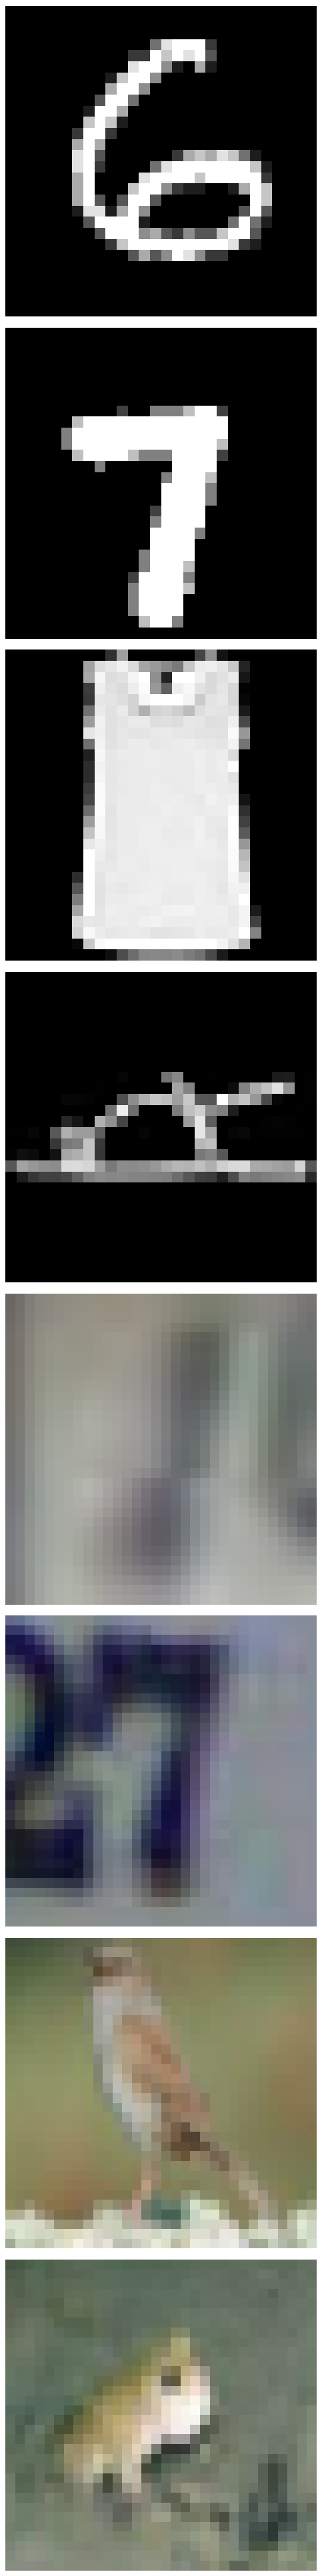
\includegraphics[width=.743478\textwidth, left]{carlini_wagner_orig_appendix.pdf}%
		\caption{Original}%
	\end{subfigure}%
	\begin{subfigure}{.36\textwidth}
		\centering
		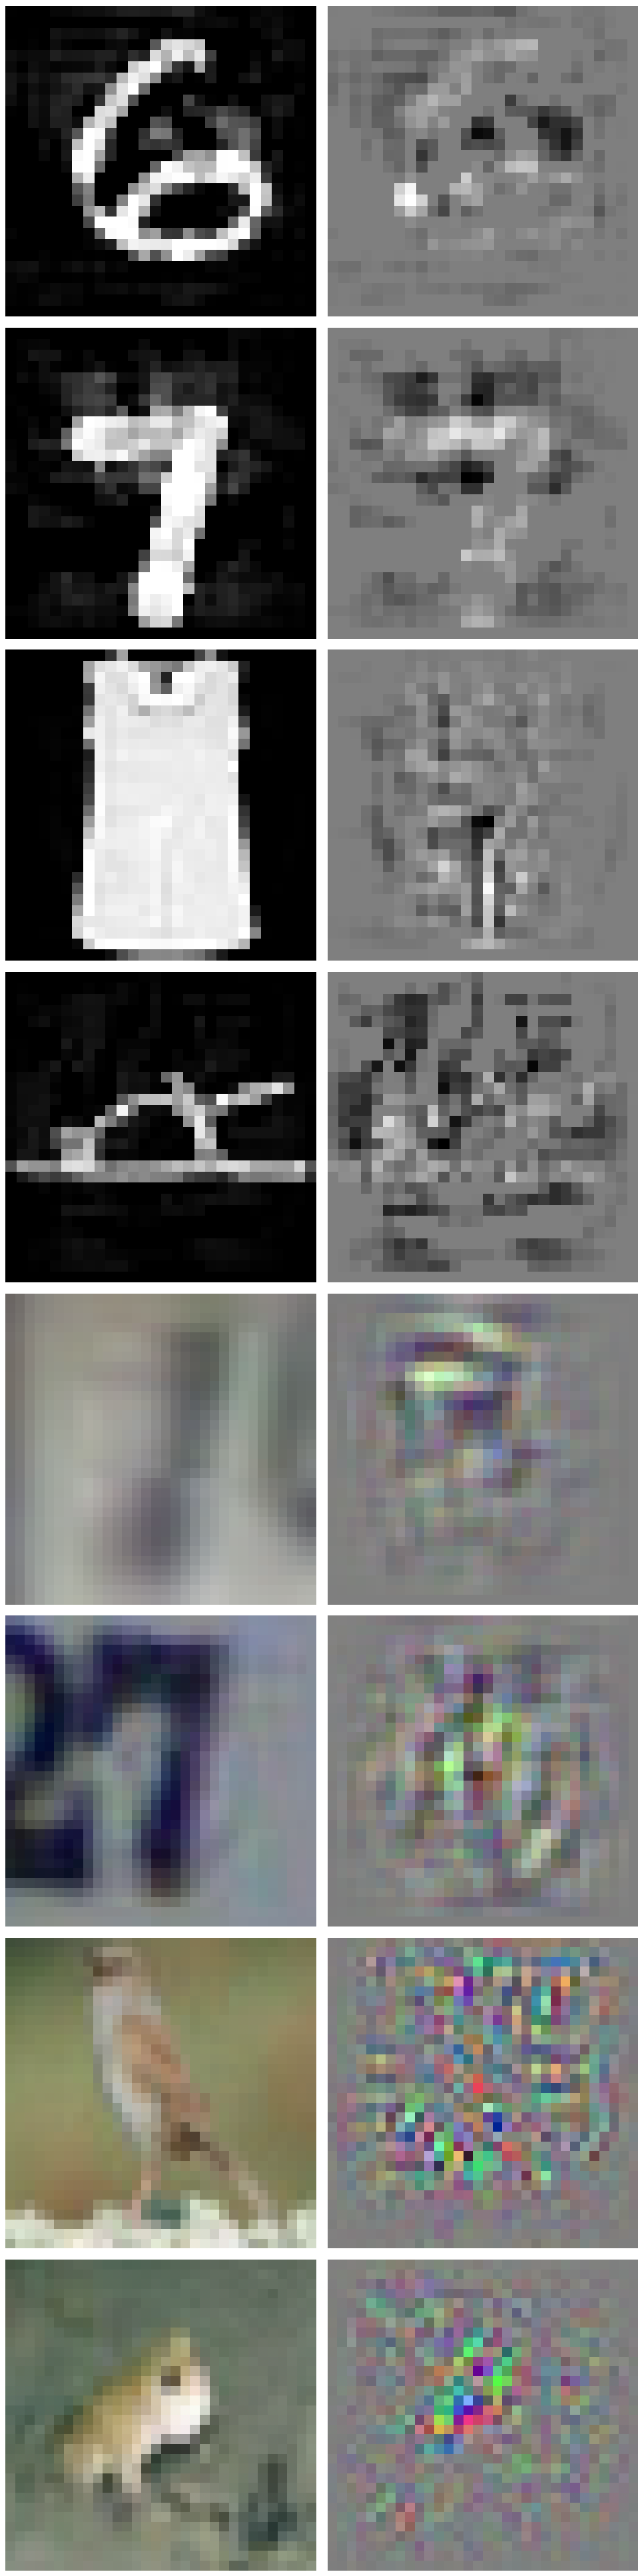
\includegraphics[width=.95\textwidth, center]{carlini_wagner_caps_appendix.pdf}%
		\caption{CapsNet}
	\end{subfigure}%
	\begin{subfigure}{.36\textwidth}
		\centering
		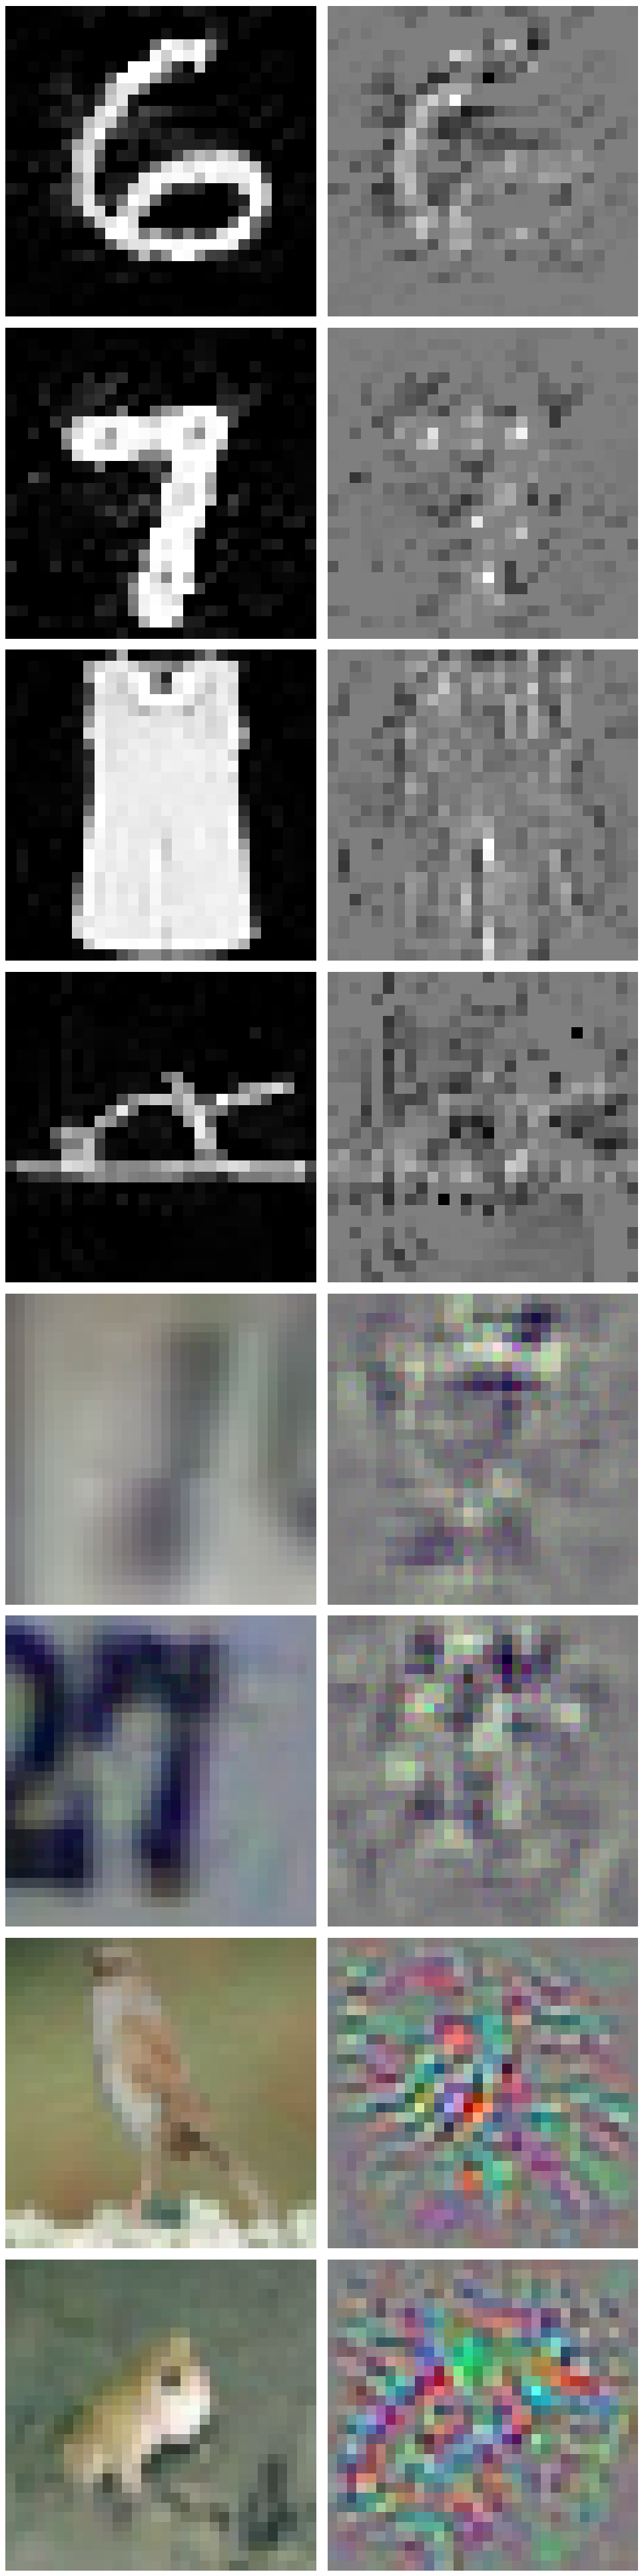
\includegraphics[width=.95\textwidth, right]{carlini_wagner_conv_appendix.pdf}%
		\caption{ConvNet}
	\end{subfigure}
	\caption[Carlini-Wagner Adversarial Examples]{Carlini-Wagner adversarial examples and perturbations. Pixel values of perturbation images are scaled for visibility}
	\label{fig:carlini-wagner-img}
	
\end{figure}


\begin{figure}
	\centering
	
	\begin{subfigure}{.23\textwidth}
		\centering
		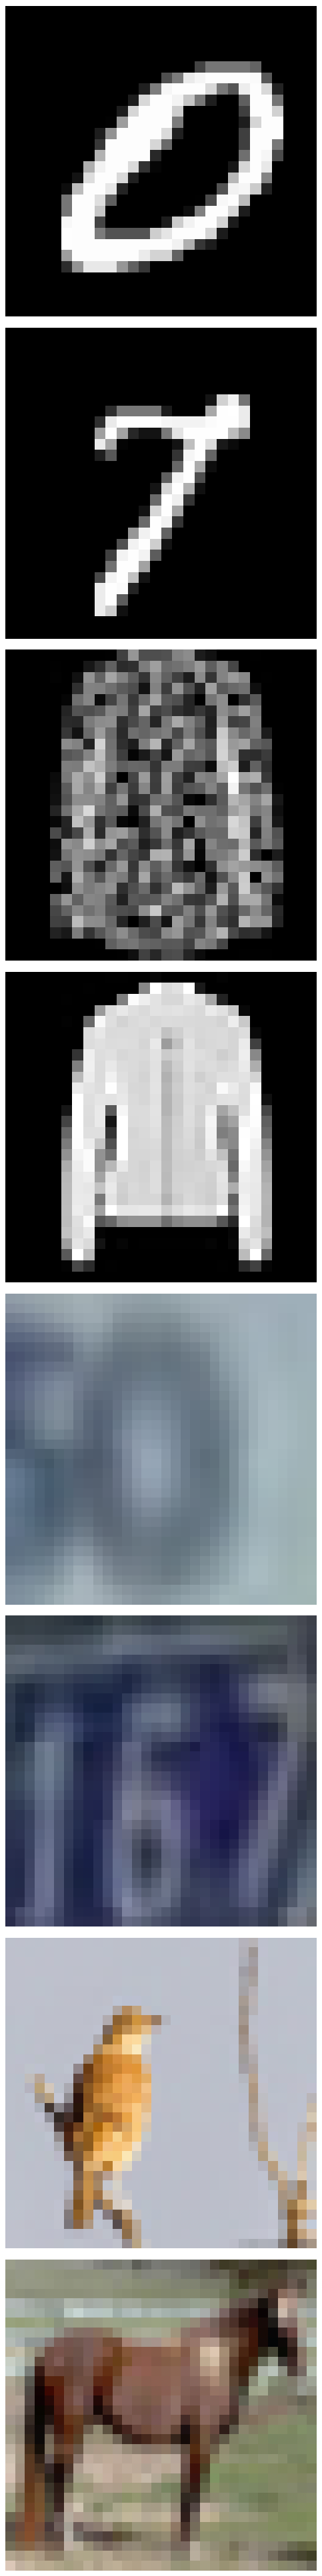
\includegraphics[width=.743478\textwidth, left]{deepfool_orig_appendix.pdf}%
		\caption{Original}%
	\end{subfigure}%
	\begin{subfigure}{.36\textwidth}
		\centering
		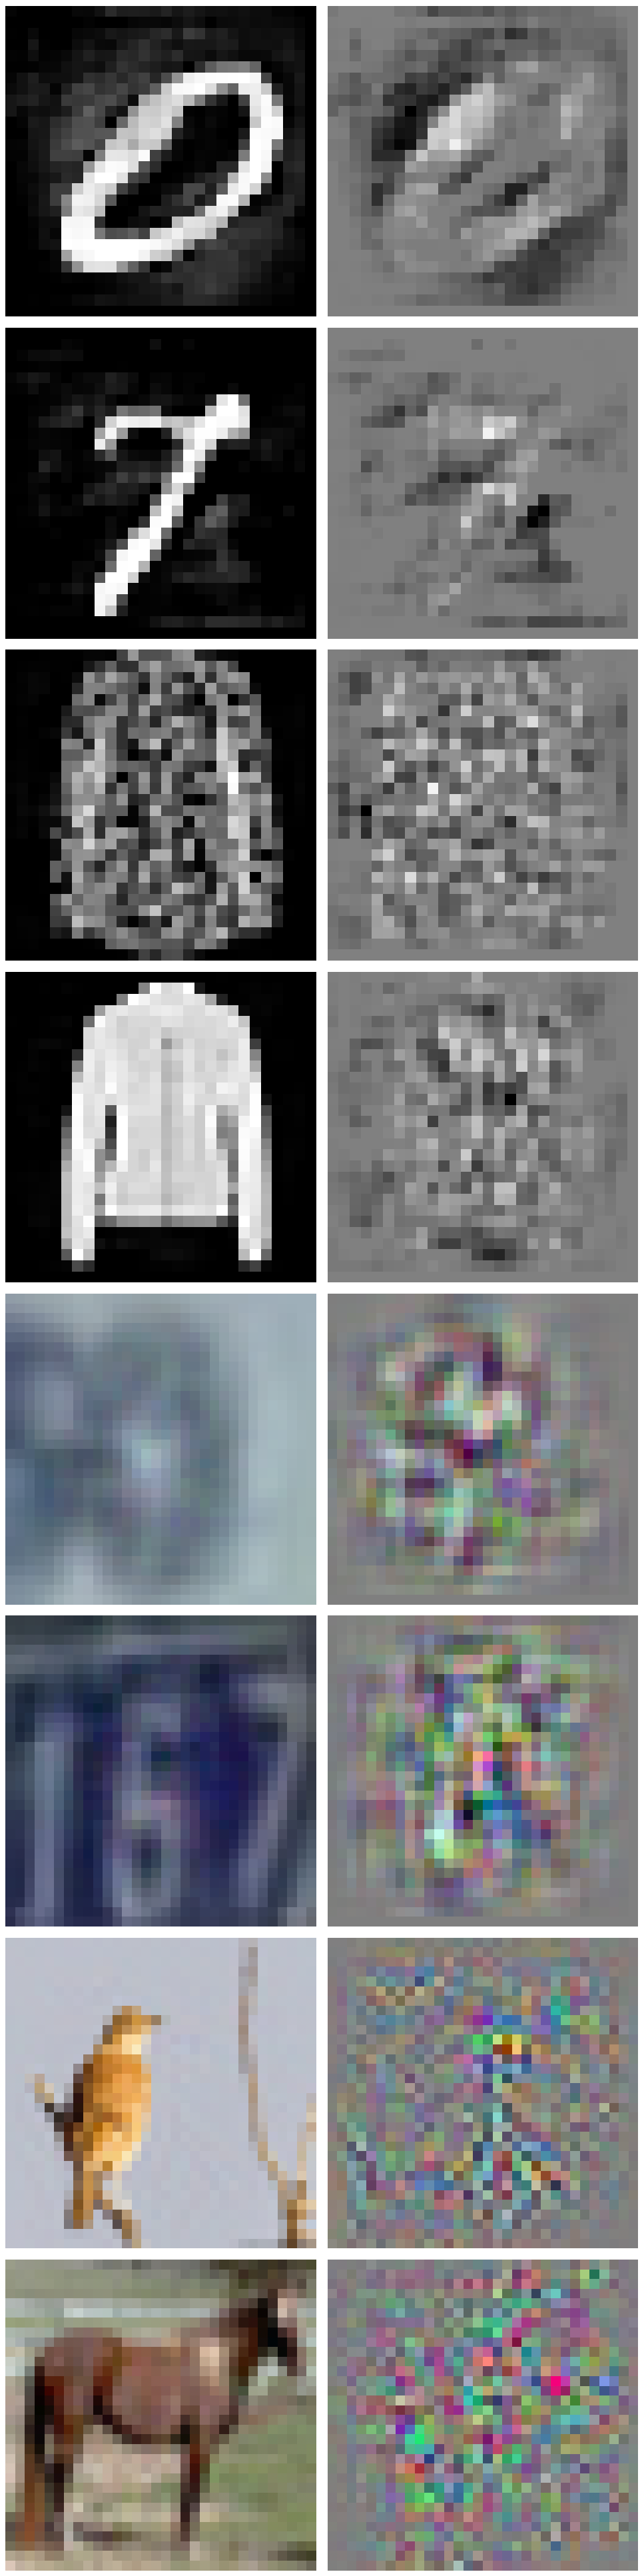
\includegraphics[width=.95\textwidth, center]{deepfool_caps_appendix.pdf}%
		\caption{CapsNet}
	\end{subfigure}%
	\begin{subfigure}{.36\textwidth}
		\centering
		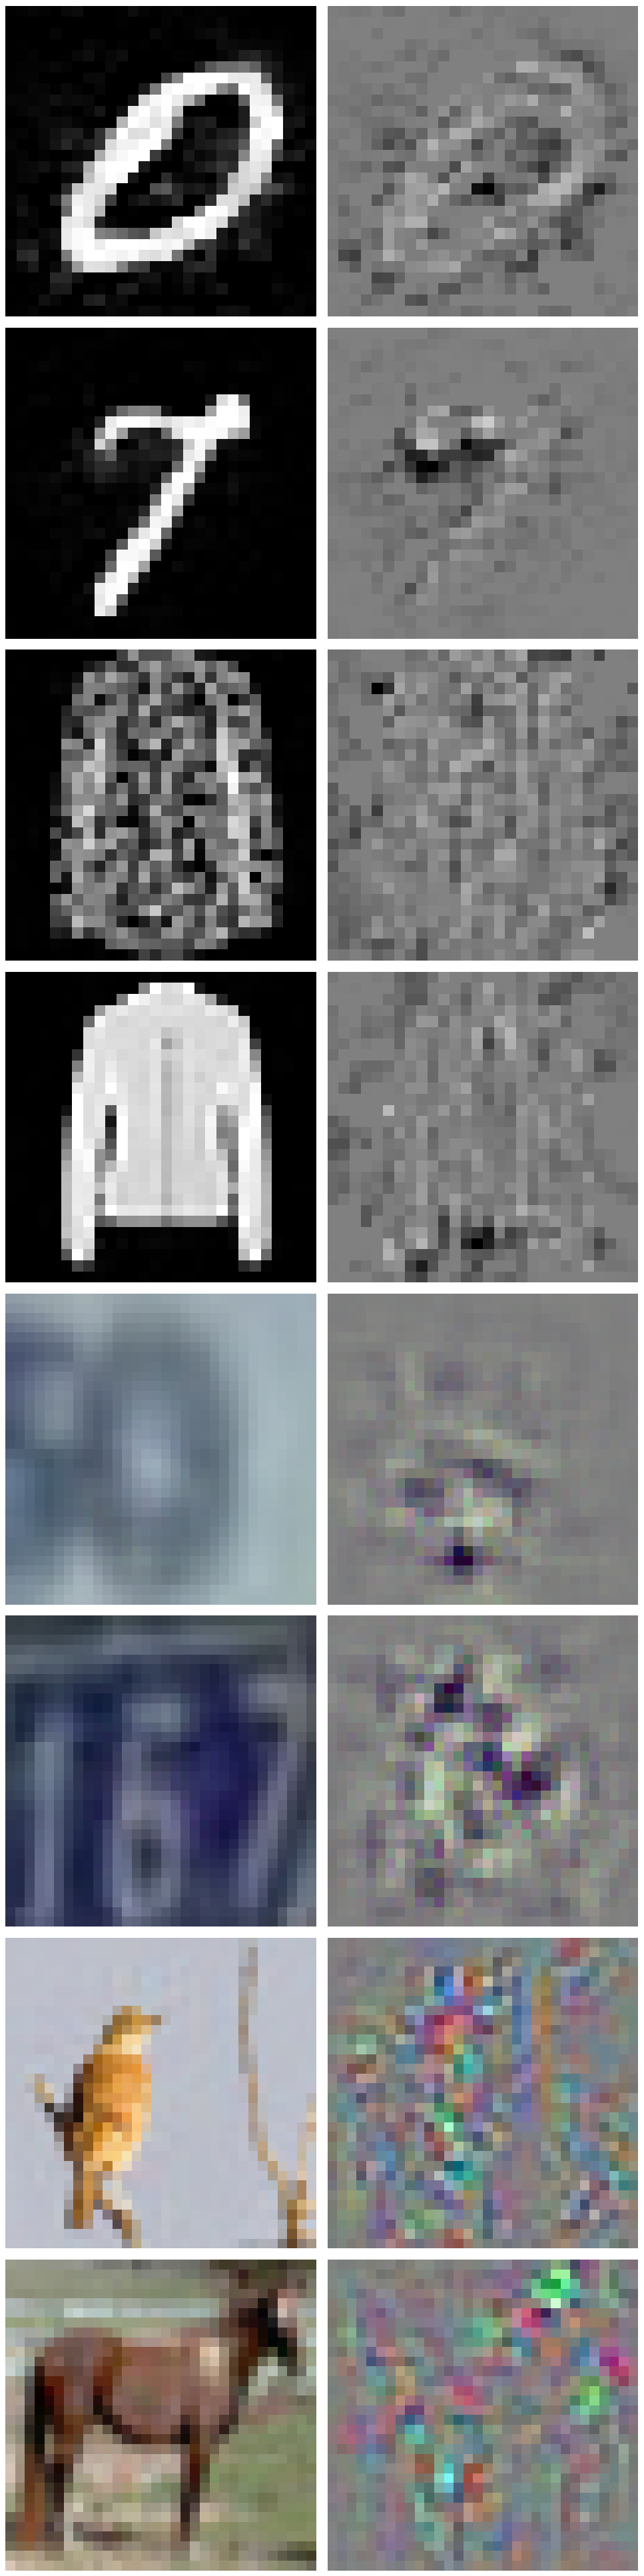
\includegraphics[width=.95\textwidth, right]{deepfool_conv_appendix.pdf}%
		\caption{ConvNet}
	\end{subfigure}
	\caption[DeepFool Adversarial Examples]{DeepFool adversarial examples and perturbations. Pixel values of perturbation images are scaled for visibility}
	\label{fig:deepfool-img}
	
\end{figure}

\begin{figure}
	\centering
	
	\begin{subfigure}{.23\textwidth}
		\centering
		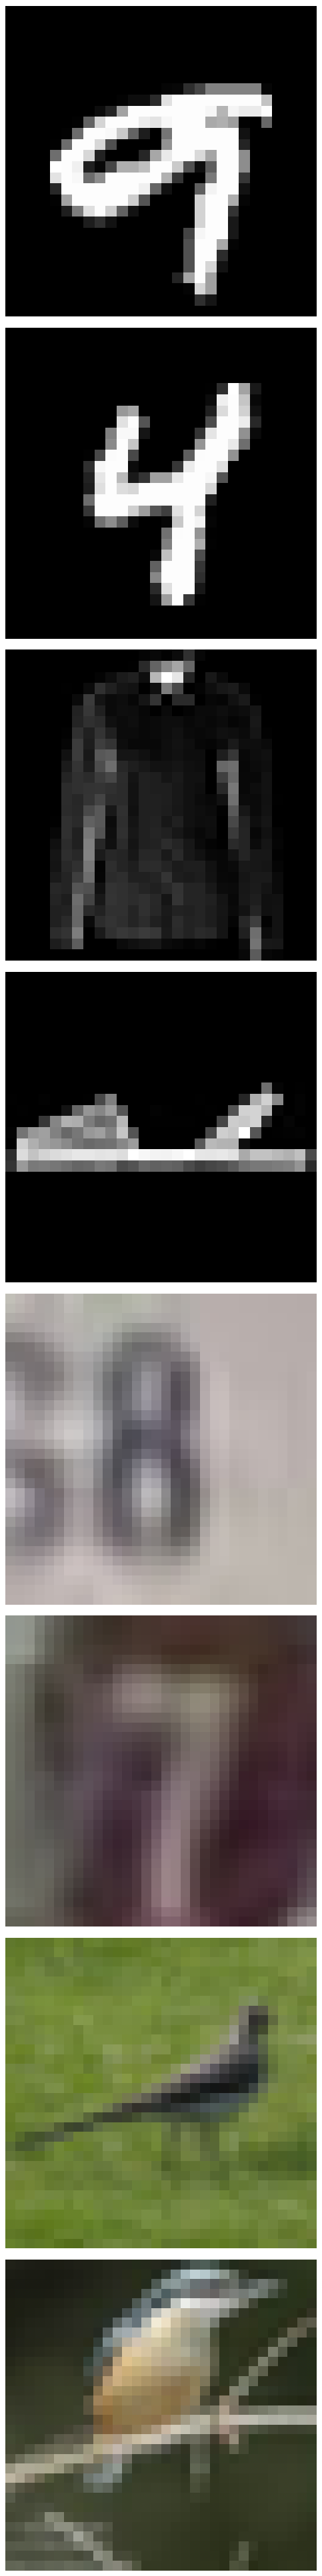
\includegraphics[width=.743478\textwidth, left]{boundary_attack_orig_appendix.pdf}%
		\caption{Original}%
	\end{subfigure}%
	\begin{subfigure}{.36\textwidth}
		\centering
		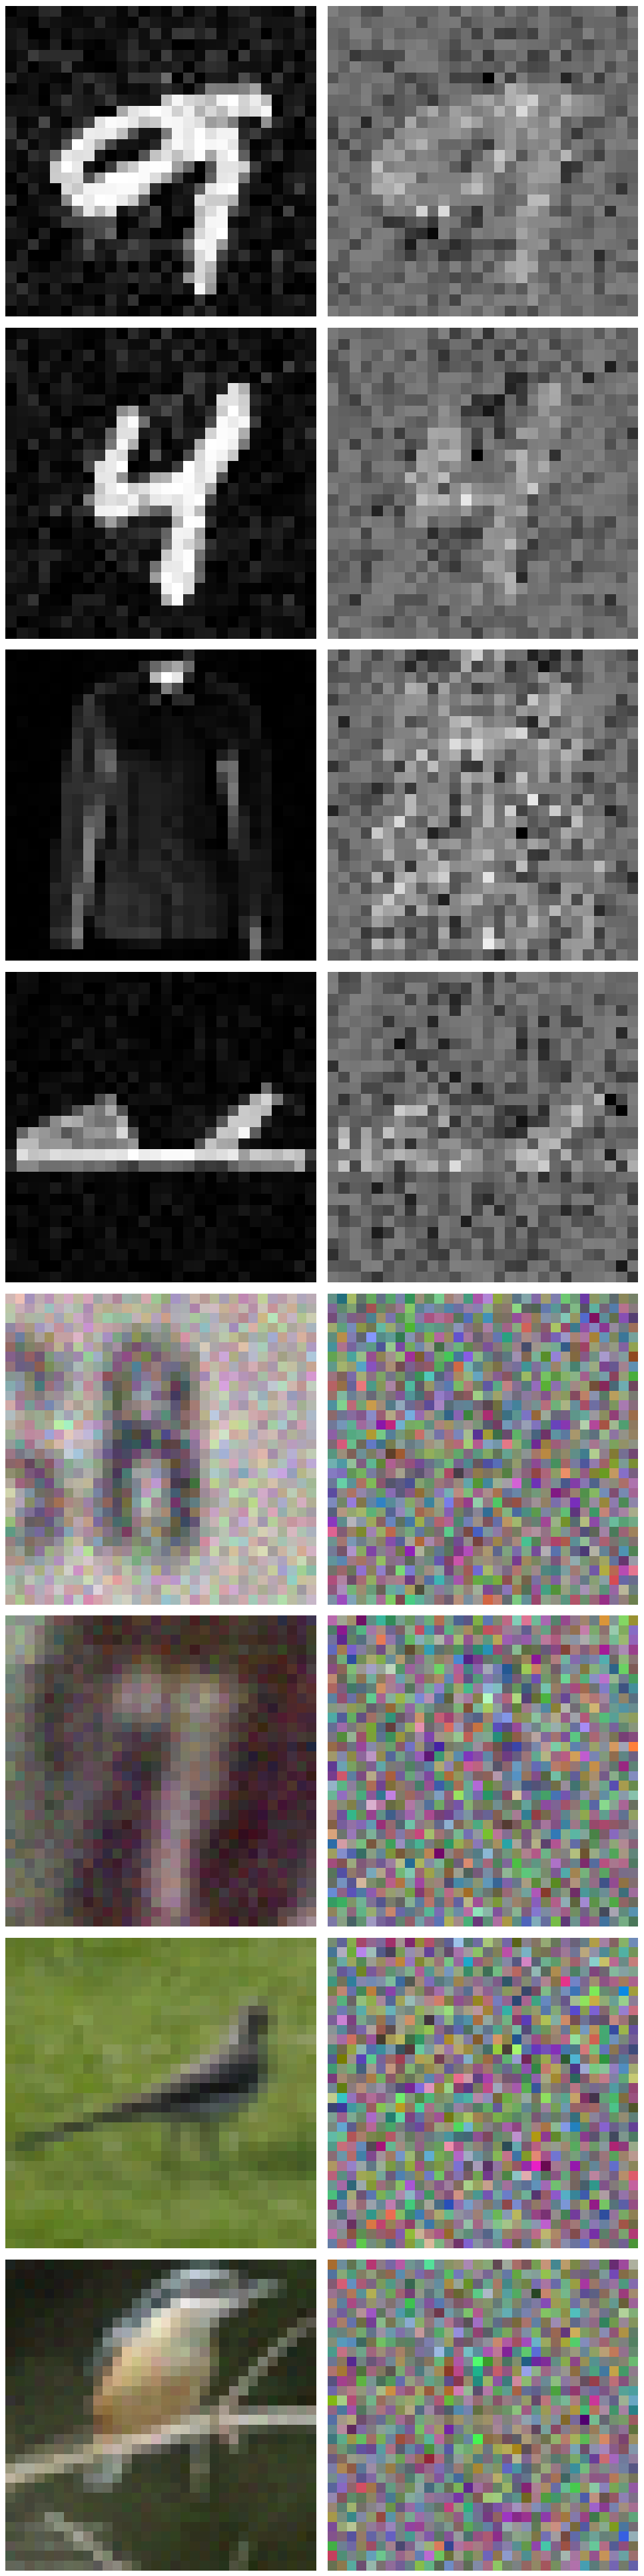
\includegraphics[width=.95\textwidth, center]{boundary_attack_caps_appendix.pdf}%
		\caption{CapsNet}
	\end{subfigure}%
	\begin{subfigure}{.36\textwidth}
		\centering
		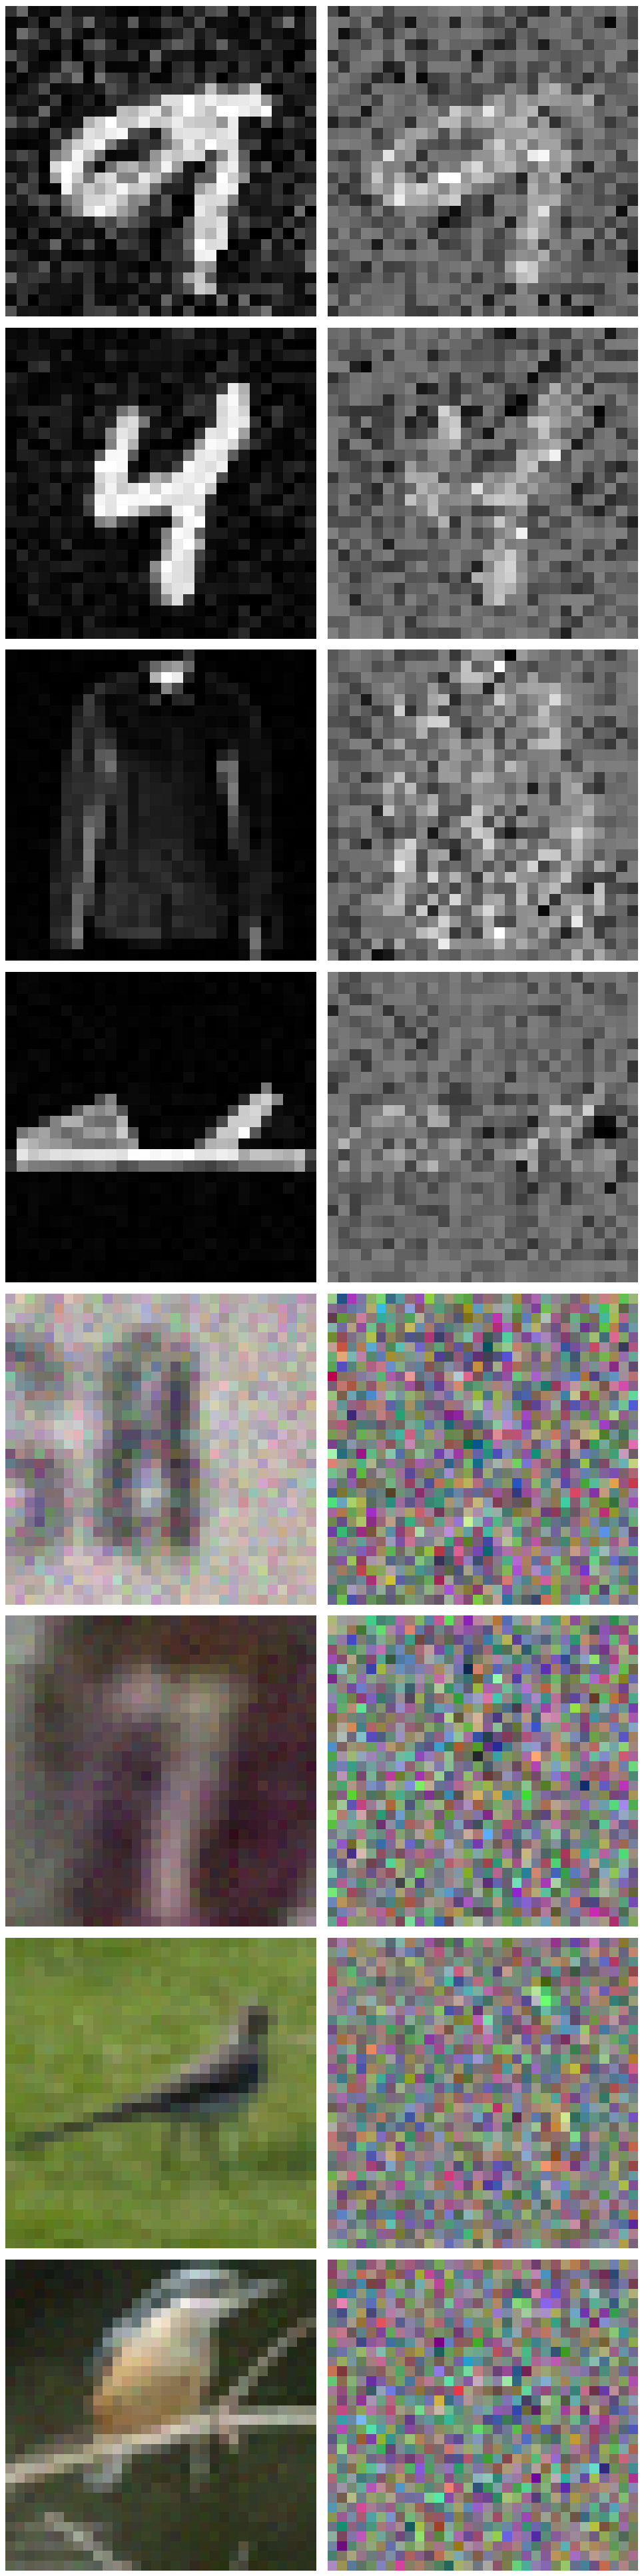
\includegraphics[width=.95\textwidth, right]{boundary_attack_conv_appendix.pdf}%
		\caption{ConvNet}
	\end{subfigure}
	\caption[Boundary Attack Adversarial Examples]{Boundary Attack adversarial examples and perturbations. Pixel values of perturbation images are scaled for visibility}
	\label{fig:boundary-img}
	
\end{figure}

\begin{figure}
	\centering
	
	\begin{subfigure}{.23\textwidth}
		\centering
		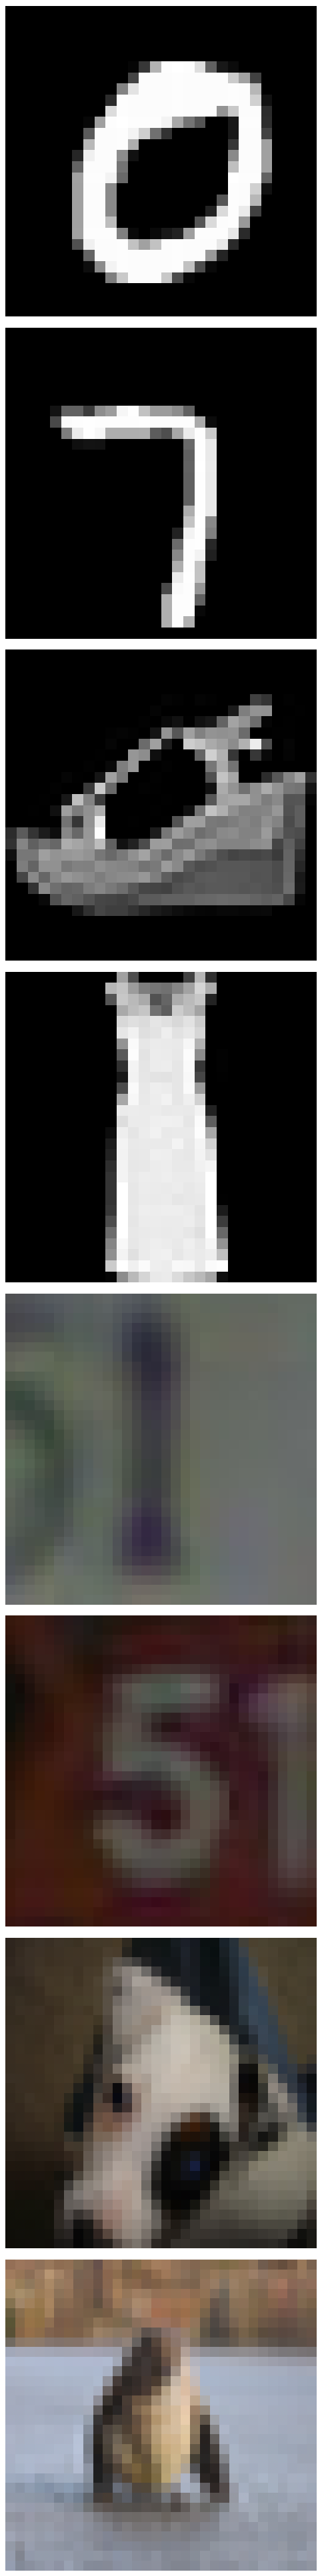
\includegraphics[width=.743478\textwidth, left]{universal_perturbation_orig_appendix.pdf}%
		\caption{Original}%
	\end{subfigure}%
	\begin{subfigure}{.36\textwidth}
		\centering
		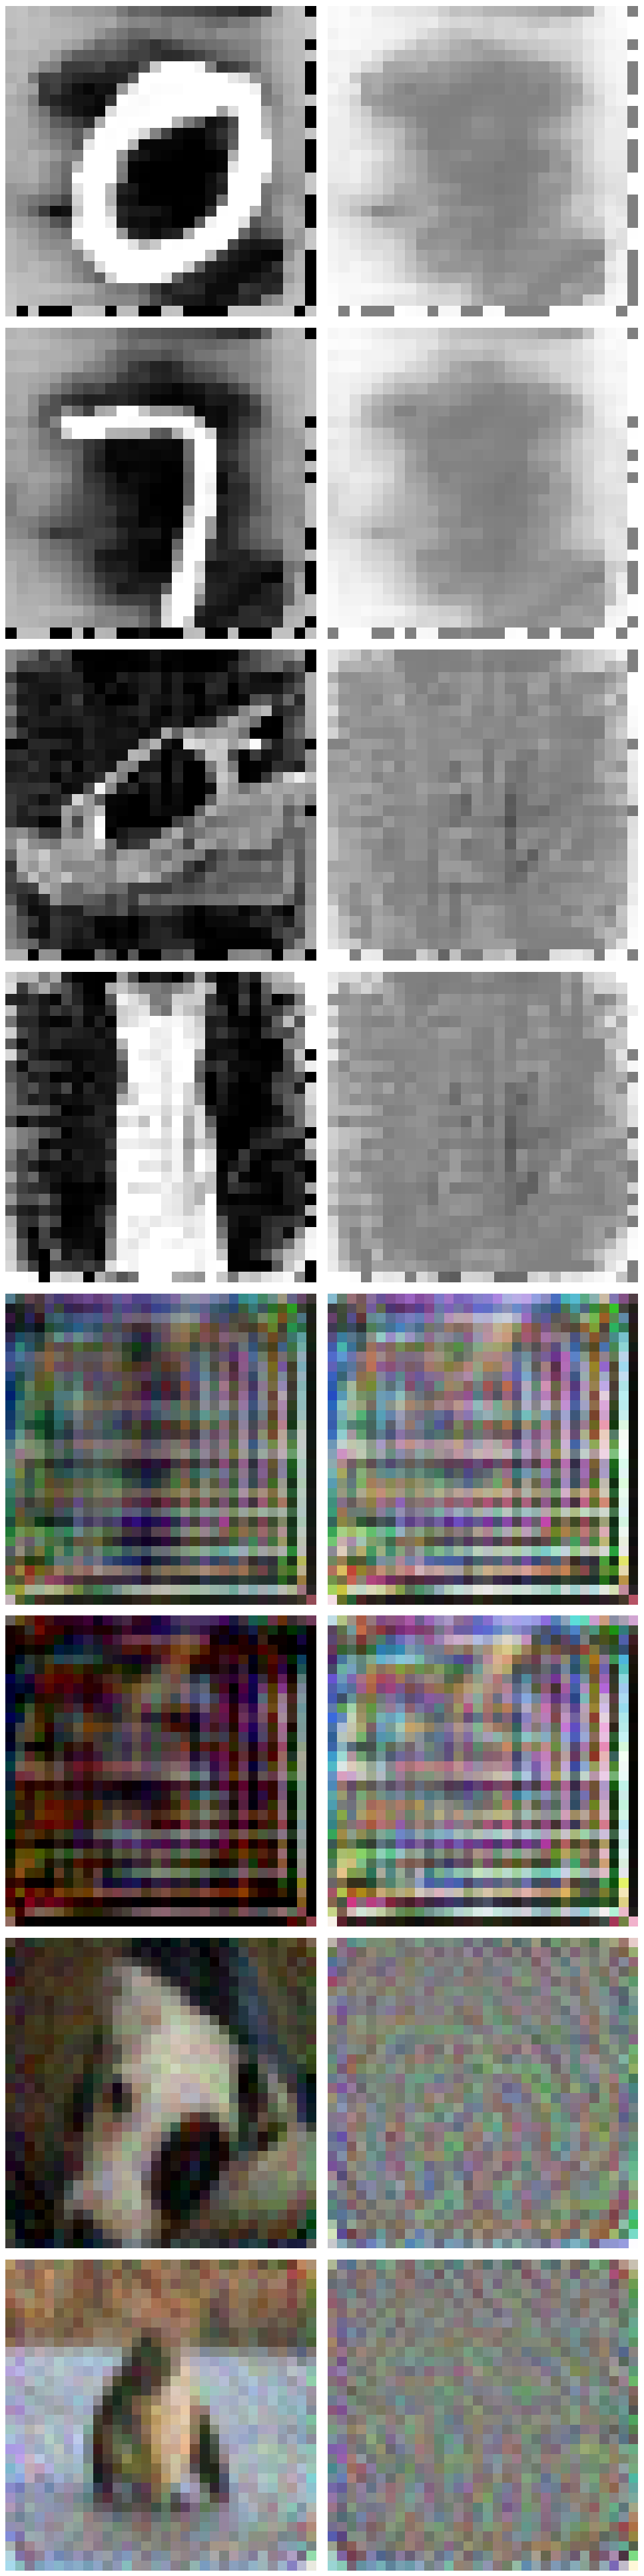
\includegraphics[width=.95\textwidth, center]{universal_perturbation_caps_appendix.pdf}%
		\caption{CapsNet}
	\end{subfigure}%
	\begin{subfigure}{.36\textwidth}
		\centering
		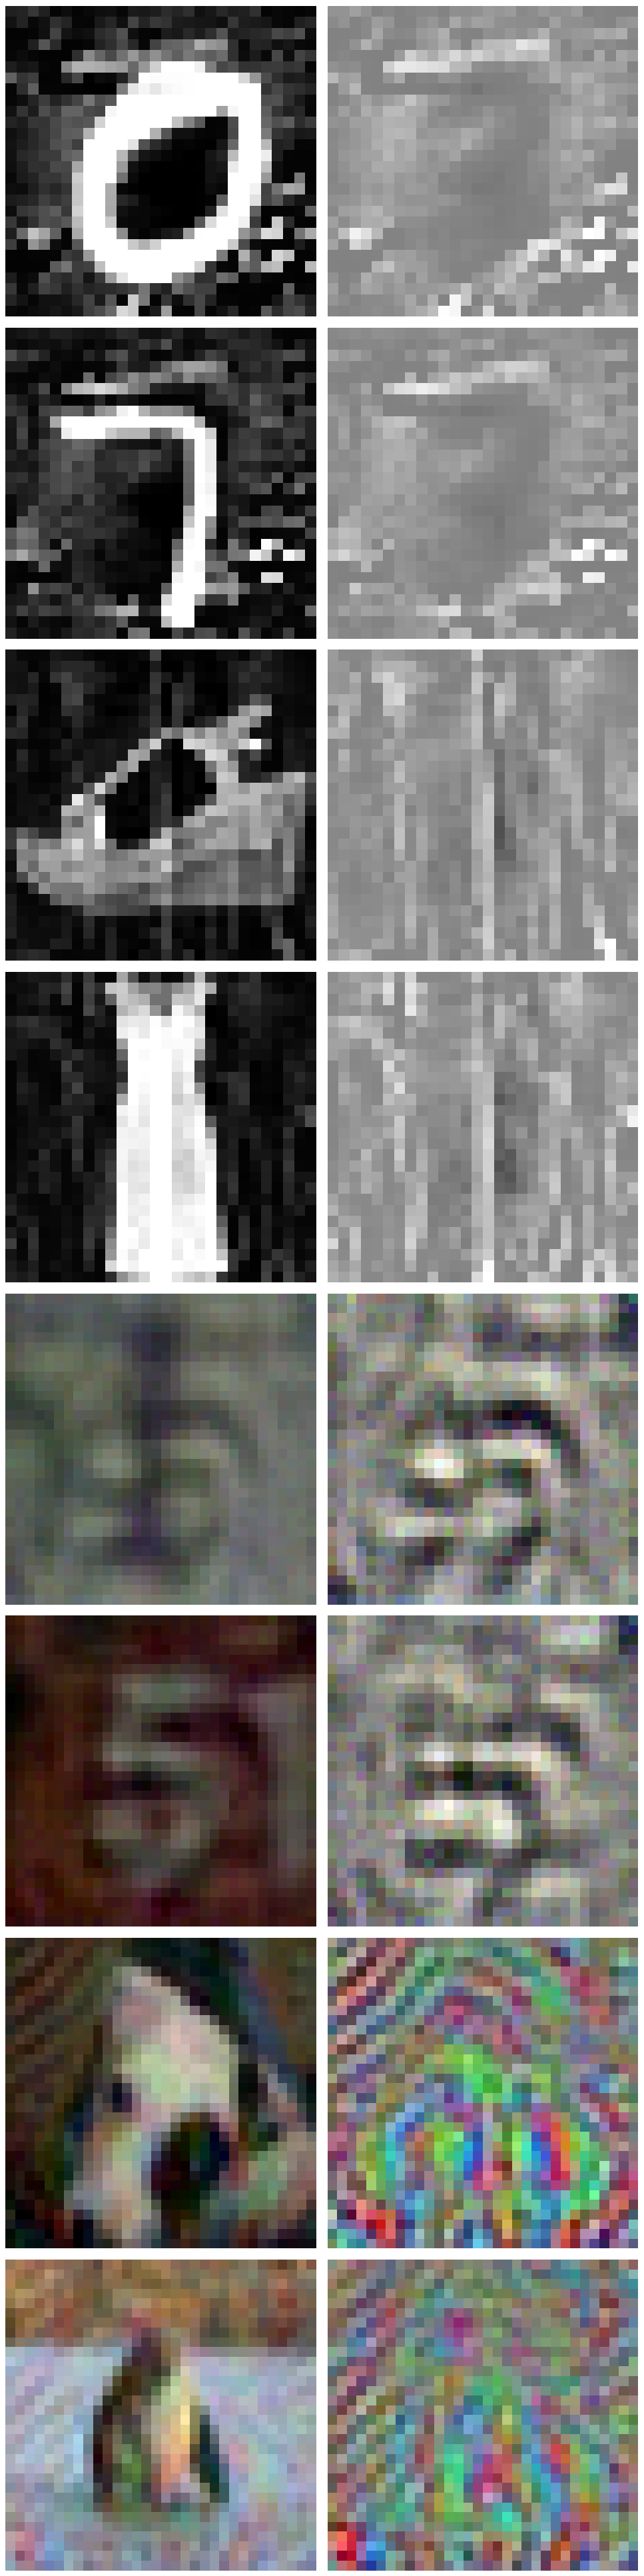
\includegraphics[width=.95\textwidth, right]{universal_perturbation_conv_appendix.pdf}%
		\caption{ConvNet}
	\end{subfigure}
	\caption[Universal Adversarial Perturbation Adversarial Examples]{Universal Adversarial Perturbation adversarial examples and perturbations. Pixel values of perturbation images are scaled for visibility}
	\label{fig:universal-img}
	
\end{figure}

\subsection{ICML Paper}

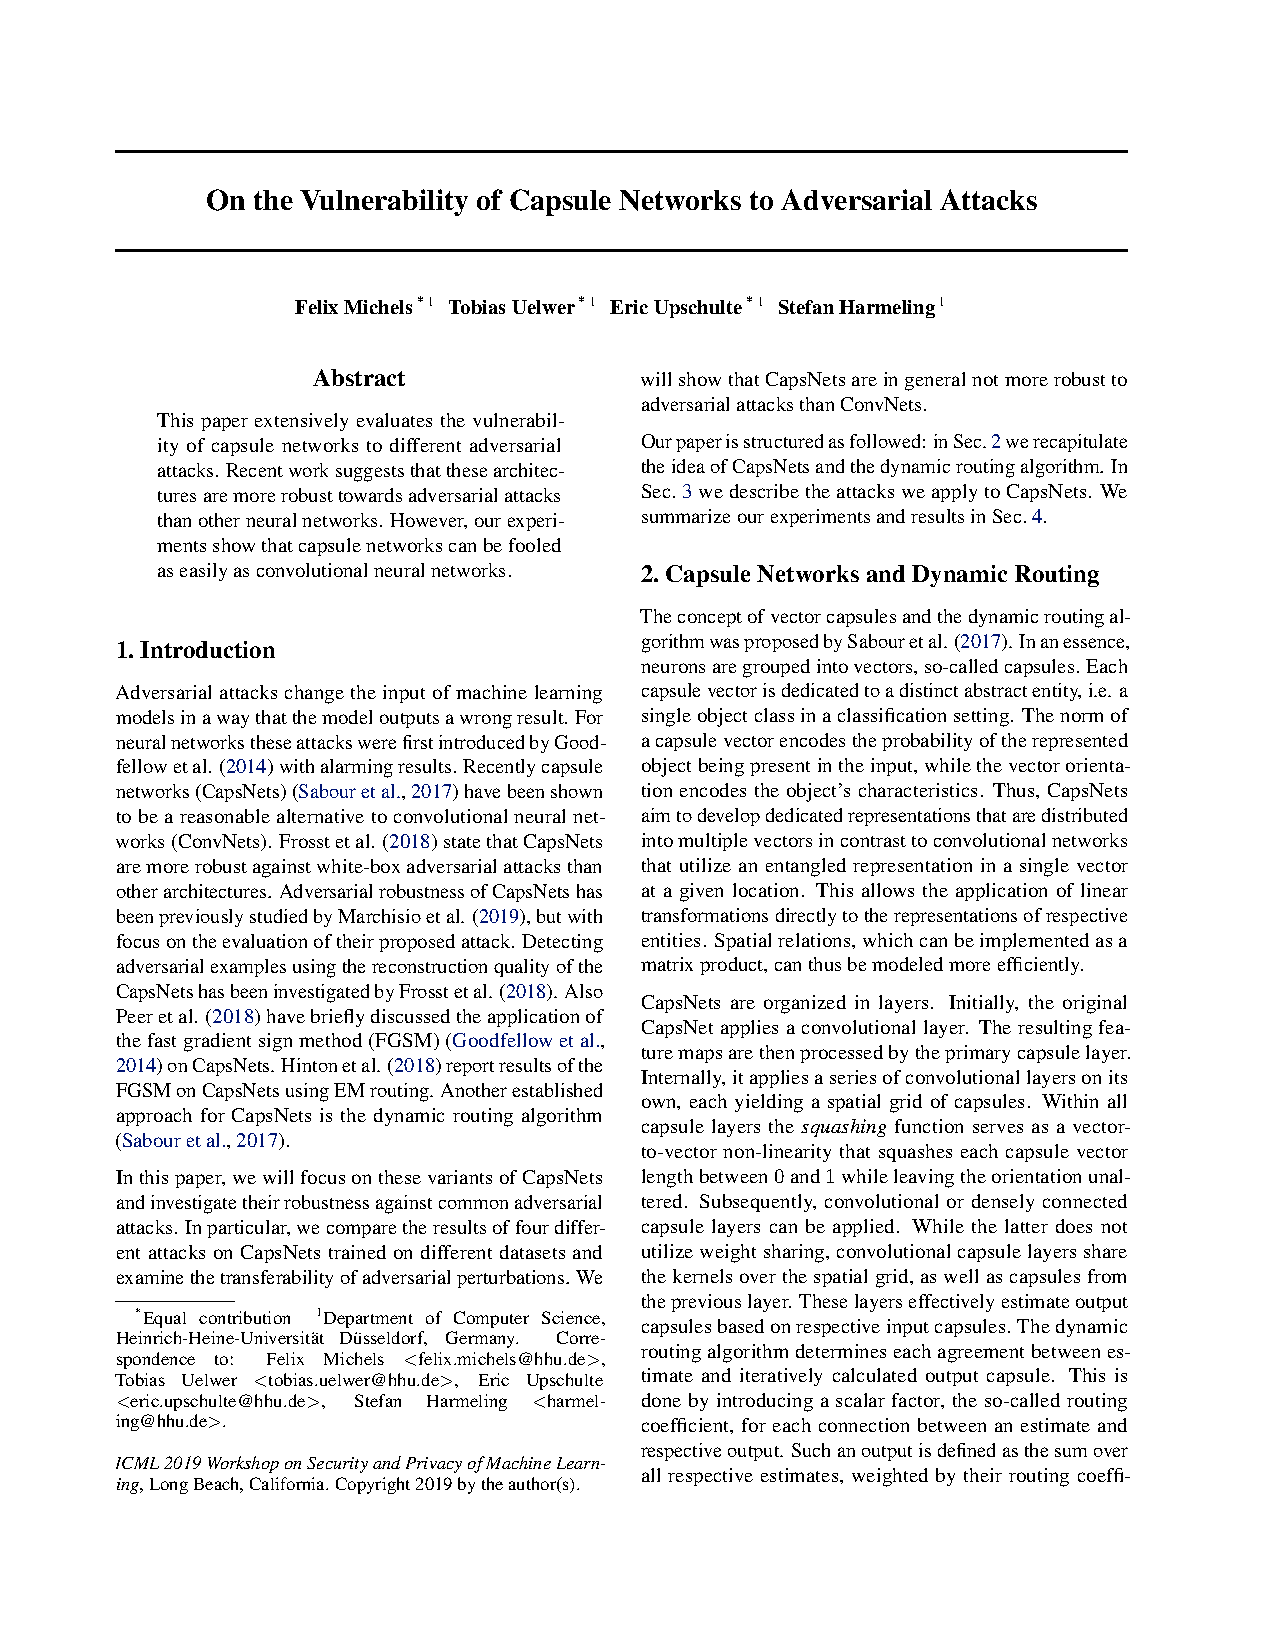
\includepdf[pages={1-4}, nup=2x2]{icml.pdf}